\chapter{Attention Mechanisms and Transformers \cite{dnn-1}} \label{Attention Mechanisms and Transformers}

SEE: \fullref{Encoder–Decoder Architecture}

\begin{enumerate}
    \item The intuition behind \textbf{attention} is that rather than compressing the input, it might be better for the decoder to revisit the input sequence at every step. 
    
    \item Moreover, rather than always seeing the same representation of the input, one might imagine that the decoder should selectively focus on particular parts of the input sequence at particular decoding steps. 
    
    \item Bahdanau’s attention mechanism provided a simple means by which the decoder could dynamically attend to different parts of the input at each decoding step. 
    
    \item The high-level idea is that the encoder could produce a representation of length equal to the original input sequence. \\
    Then, at decoding time, the decoder can (via some control mechanism) receive as input a context vector consisting of a weighted sum of the representations on the input at each time step. 
    
    \item Intuitively, the weights determine the extent to which each step’s context “focuses” on each input token, and the key is to make this process for assigning the weights differentiable so that it can be learned along with all of the other neural network parameters.

    \item The insights spurred claims that attention models confer “interpretability” although what precisely the attention weights mean—i.e., how, if at all, they should be interpreted remains a hazy research topic.

    \item \textbf{Transformer architecture} for machine translation, dispensing with recurrent connections altogether, and instead relying on cleverly arranged attention mechanisms to capture all relationships among input and output tokens. 
    
\end{enumerate}


\section{Queries, Keys, and Values \cite{dnn-1}}

\begin{figure}[H]
    \centering
    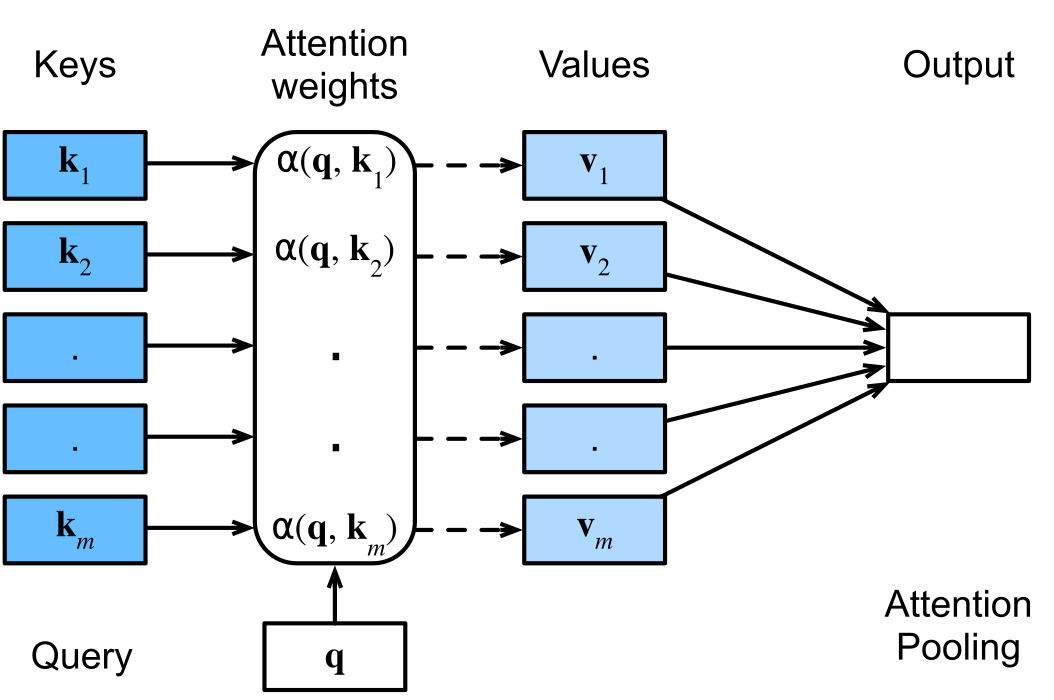
\includegraphics[width=\linewidth, height=4cm, keepaspectratio]{Pictures/deep_neural_networks/attention-qkv.jpg}
    \caption*{The attention mechanism computes a linear combination over values $\mathbf{v}_\mathit{i}$ via attention pooling, where weights are derived according to the compatibility between a query $\mathbf{q}$ and keys $\mathbf{k}_\mathit{i}$.}
\end{figure}

\begin{customTableWrapper}{1.5}
\begin{longtable}{l p{8cm}}
    $\mathcal{D}$ & database (lookup key-value pairs) \\

    $k$ or $\mathbf{k}_i$ & Key \\

    $v$ or $\mathbf{v}_i$ & Value \\

    $m$ & number of key-value pairs in $\mathcal{D}$ \\

    $q$ or $\mathbf{q}$ & query \\

    $\alpha(\mathbf{q}, \mathbf{k}_i) \in \mathbb{R}$ & scalar attention weights \\

\end{longtable}
\end{customTableWrapper}

\begin{enumerate}[itemsep=0.15cm]
    \item $\mathcal{D} \stackrel{\textrm{def}}{=} \{(\mathbf{k}_1, \mathbf{v}_1), \ldots (\mathbf{k}_m, \mathbf{v}_m)\}$

    \item We can operate on $\mathcal{D}$, for instance with the exact query ($q$) for $\mathbf{k}_i$ which would return the value $\mathbf{v}_i$. 
    
    \item If $(\mathbf{k}_i, \mathbf{v}_i)$ was not a record in $\mathcal{D}$, there would be no valid answer.

    \item We can design queries $q$ that operate on $(k,v)$ pairs in such a manner as to be valid regardless of the database size

    \item The same query can receive different answers, according to the contents of the database

    \item The “code” being executed for operating on a large state space (the database) can be quite simple (e.g., exact match, approximate match, top-$k$)

    \item There is no need to compress or simplify the database to make the operations effective.

    \item attention over $\mathcal{D}$: $\textrm{Attention}(\mathbf{q}, \mathcal{D}) \stackrel{\textrm{def}}{=} \dsum_{i=1}^m \alpha(\mathbf{q}, \mathbf{k}_i) \mathbf{v}_i$
    \hfill
    (aka attention pooling)

    \item The name attention derives from the fact that the operation pays particular attention to the terms for which the weight $\alpha$ is significant (i.e., large). 
    
    \item The attention over $\mathcal{D}$ generates a linear combination of values contained in the database.

    \item \textbf{special cases}:
    \begin{enumerate}[itemsep=0.1cm]
        \item The weights $\alpha(\mathbf{q}, \mathbf{k}_i)$ are nonnegative.\\
        In this case the output of the attention mechanism is contained in the convex cone spanned by the values $\mathbf{v}_i$

        \item The weights $\alpha(\mathbf{q}, \mathbf{k}_i)$ form a convex combination, i.e., $\dsum_i \alpha(\mathbf{q}, \mathbf{k}_i) = 1$ and $\alpha(\mathbf{q}, \mathbf{k}_i) \geq 0$ for all $i$.\\
        This is the most common setting in deep learning.

        \item Exactly one of the weights $\alpha(\mathbf{q}, \mathbf{k}_i)$ is $i$, while all others are $0$.\\
        This is akin to a traditional database query.

        \item All weights are equal, i.e., $\alpha(\mathbf{q}, \mathbf{k}_i) = \dfrac{1}{m}$ for all $i$.\\
        This amounts to averaging across the entire database, also called average pooling in deep learning.
    \end{enumerate}

    \item A common strategy for ensuring that the weights sum up to 1 is to normalize them via
    $
        \alpha(\mathbf{q}, \mathbf{k}_i) = \dfrac{\alpha(\mathbf{q}, \mathbf{k}_i)}{{\dsum_j} \alpha(\mathbf{q}, \mathbf{k}_j)}
    $

    \item to ensure that the weights are also nonnegative, we can use exponentiation.\\
    This means that we can now pick any function $a(\mathbf{q}, \mathbf{k})$ and then apply the softmax operation used for multinomial models to it via
    $
        \alpha(\mathbf{q}, \mathbf{k}_i) = \dfrac{\exp(a(\mathbf{q}, \mathbf{k}_i))}{\dsum_j \exp(a(\mathbf{q}, \mathbf{k}_j))}
    $\\
    It is differentiable and its gradient never vanishes

\end{enumerate}



\section{Attention Pooling by Similarity \cite{dnn-1}}

SEE: \fullref{Attention VS Attention Pooling}

\begin{customTableWrapper}{1.5}
\begin{longtable}{l p{8cm}}
    $\alpha(\mathbf{q}, \mathbf{k})$ & similarity kernel \\

    
\end{longtable}
\end{customTableWrapper}

\begin{enumerate}[itemsep=0.15cm]
    \item $\alpha(\mathbf{q}, \mathbf{k})$ similarity kernel relates queries $\mathbf{q}$ to keys $\mathbf{k}$
    
    \item Common kernels:\\
    $
        \alpha(\mathbf{q}, \mathbf{k}) = 
        \renewcommand{\arraystretch}{2}
        \begin{dcases}
            \exp\left(-\dfrac{1}{2} \|\mathbf{q} - \mathbf{k}\|^2 \right) & \textrm{Gaussian} \\
            1 \textrm{ if } \|\mathbf{q} - \mathbf{k}\| \leq 1 & \textrm{Boxcar} \\
            \mathop{\mathrm{max}}\left(0, 1 - \|\mathbf{q} - \mathbf{k}\|\right) & \textrm{Epanechikov}    
        \end{dcases}
        \renewcommand{\arraystretch}{1}
    $

    \item Kernel density estimation = parzen window

    \item All of the kernels are heuristic and can be tuned\\
    For instance, we can adjust the width, not only on a global basis but even on a per-coordinate basis

    \item Regardless, all of them lead to the following equation for regression and classification alike: $f(\mathbf{q}) = \dsum_i \mathbf{v}_i \dfrac{\alpha(\mathbf{q}, \mathbf{k}_i)}{\dsum_j \alpha(\mathbf{q}, \mathbf{k}_j)}$

    \item In the case of a (scalar) regression with observations $(\mathbf{x}_i, y_i)$ for features and labels respectively, $\mathbf{v}_i = y_i$ are scalars, $\mathbf{k}_i = \mathbf{x}_i$ are vectors, and the query $\mathbf{q}$ denotes the new location where $f$ should be evaluated

    \item In the case of (multiclass) classification, we use one-hot-encoding of $y_i$ to obtain $\mathbf{v}_i$. 
    
    \item One of the convenient properties of this estimator is that it requires no training. 
    
    \item Even more so, if we suitably narrow the kernel with increasing amounts of data, the approach is consistent, i.e., it will converge to some statistically optimal solution.

    \item \textbf{translation and rotation invariant kernels}\indexlabel{translation and rotation invariant kernels}: if we shift and rotate $\mathbf{k}$ and $\mathbf{q}$ in the same manner, the value of $\alpha$ remains unchanged

    \item Different kernels correspond to different notions of range and smoothness.

    \item these are distance-based kernels\\
    distance functions are slightly more expensive to compute than dot products

\subsection{Attention Pooling via Nadaraya–Watson Regression \cite{dnn-1}}

    \item dependency: $y_i = 2\sin(x_i) + x_i + \epsilon$\\
    where $\epsilon$ is drawn from a normal distribution with zero mean and unit variance.

    \item we also want to obtain the relative kernel weights in order to perform some minor diagnostics.\\
    Hence we first compute the kernel between all training features (covariates) \verb|x_train| and all validation features \verb|x_val|.\\
    This yields a matrix, which we subsequently normalize.\\
    When multiplied with the training labels \verb|y_train| we obtain the estimates.

    \item Let each validation feature be a query, and each training feature–label pair be a key–value pair.\\
    As a result, the normalized relative kernel weights are the \textbf{attention weights}.

\subsection{Adapting Attention Pooling \cite{dnn-1}}

    \item $\alpha(\mathbf{q}, \mathbf{k}) = \exp\left(-\dfrac{1}{2 \sigma^2} \|\mathbf{q} - \mathbf{k}\|^2 \right)$

    \item $\sigma^2$ = width of the kernel

    \item the narrower the kernel, the less smooth the estimate. At the same time, it adapts better to the local variations.
    
\end{enumerate}


\section{Attention Scoring Functions \cite{dnn-1}} \label{Attention Scoring Functions}

\begin{figure}[H]
    \centering
    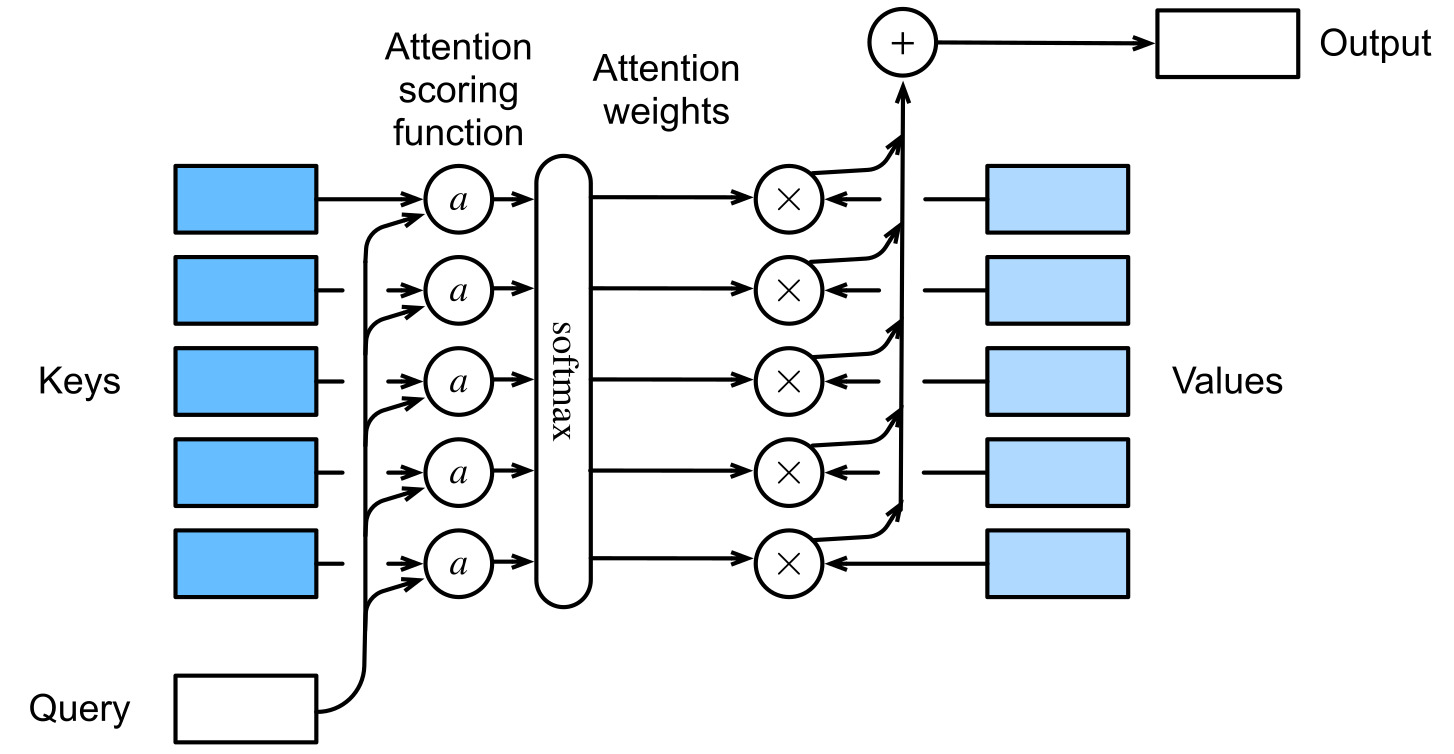
\includegraphics[width=\linewidth, height=5cm, keepaspectratio]{Pictures/deep_neural_networks/Attention-Scoring-Function.jpg}
    \caption*{Computing the output of attention pooling as a weighted average of values, where weights are computed with the attention scoring function $\alpha$ and the softmax operation.}
\end{figure}

\begin{enumerate}
    \item compared to distance-based kernels, attention scoring functions are simpler to compute

    
\end{enumerate}

\subsection{Dot Product Attention \cite{dnn-1}} \label{Dot Product Attention}

\begin{enumerate}[itemsep=0.15cm]
    \item Assume that all the elements of the query $\mathbf{q} \in \mathbb{R}^d$ and the key $\mathbf{k}_i \in \mathbb{R}^d$ are independent and identically drawn random variables with zero mean and unit variance.\\
    The dot product between both vectors has zero mean and a variance of $d$\\
    To ensure that the variance of the dot product still remains $1$ regardless of vector length, we use the scaled dot product attention scoring function.

    \item attention function (without exponentiation) from the Gaussian kernel: 
    \item[] $
        \hfill
        a(\mathbf{q}, \mathbf{k}_i) = -\dfrac{1}{2} \|\mathbf{q} - \mathbf{k}_i\|^2  = \mathbf{q}^\top \mathbf{k}_i -\dfrac{1}{2} \|\mathbf{k}_i\|^2  -\dfrac{1}{2} \|\mathbf{q}\|^2
        \hfill
    $
    \begin{enumerate}
        \item final term depends on $\mathbf{q}$ only\\
        it is identical for all $(\mathbf{q}, \mathbf{k}_i)$ pairs.\\
        Normalizing the attention weights to $1$ ensures that this term disappears entirely

        \item both batch and layer normalization (to be discussed later) lead to activations that have well-bounded, and often constant, norms $\|\mathbf{k}_i\|$\\
        we can drop it from the definition of $\alpha$ without any major change in the outcome

        
    \end{enumerate}

    \item we rescale the dot product by $1/\sqrt{d}$. \\
    We thus arrive at the first commonly used attention function that is used, e.g., in Transformers $a(\mathbf{q}, \mathbf{k}_i) = \mathbf{q}^\top \mathbf{k}_i / \sqrt{d}$

    \item attention weights $\alpha$ still need normalizing\\
    We can simplify this further by using the softmax operation:
    $
        \alpha(\mathbf{q}, \mathbf{k}_i) = \mathrm{softmax}(a(\mathbf{q}, \mathbf{k}_i)) = \dfrac{\exp(\mathbf{q}^\top \mathbf{k}_i / \sqrt{d})}{\dsum_{j=1} \exp(\mathbf{q}^\top \mathbf{k}_j / \sqrt{d})}
    $
\end{enumerate}


\subsection{Convenience Functions \cite{dnn-1}}

\subsubsection{Masked Softmax Operation \cite{dnn-1}}

\begin{enumerate}
    \item we need to be able to deal with sequences of different lengths\\
    such sequences may end up in the same minibatch, necessitating padding with dummy tokens for shorter sequences\\
    These special tokens do not carry meaning

\begin{lstlisting}[numbers=none]
Dive  into  Deep    Learning
Learn to    code    <blank>
Hello world <blank> <blank>
\end{lstlisting}
    
    \item Since we do not want blanks in our attention model we simply need to limit $\sum_{i=1}^n \alpha(\mathbf{q}, \mathbf{k}_i) \mathbf{v}_i$ to $\sum_{i=1}^l \alpha(\mathbf{q}, \mathbf{k}_i) \mathbf{v}_i$ for however long, $l \leq n$ the actual sentence is. \\
    Since it is such a common problem, it has a name: the masked softmax operation.

    
\end{enumerate}


\subsubsection{Batch Matrix Multiplication \cite{dnn-1}}



\begin{enumerate}
    \item[] $\mathbf{Q} = [\mathbf{Q}_1, \mathbf{Q}_2, \ldots, \mathbf{Q}_n]  \in \mathbb{R}^{n \times a \times b}$
    
    \item[] $\mathbf{K} = [\mathbf{K}_1, \mathbf{K}_2, \ldots, \mathbf{K}_n]  \in \mathbb{R}^{n \times b \times c}$

    \item multiply batches of matrices by one another

    \item This comes in handy when we have minibatches of queries, keys, and values

    \item batch matrix multiplication (BMM) computes the elementwise product:
    \[
        \hfill
        \textrm{BMM}(\mathbf{Q}, \mathbf{K}) = [\mathbf{Q}_1 \mathbf{K}_1, \mathbf{Q}_2 \mathbf{K}_2, \ldots, \mathbf{Q}_n \mathbf{K}_n] \in \mathbb{R}^{n \times a \times c}
        \hfill
    \]

\end{enumerate}


\subsection{Scaled Dot Product Attention \cite{dnn-1}}

\begin{customTableWrapper}{1.5}
\begin{longtable}{l p{8cm}}
    $n$ & number of queries \\

    $m$ & number of key-value pairs \\

    $d$ & length of keys \\

    $v$ & length of values \\

    \hline

    $\mathbf Q\in\mathbb R^{n\times d}$ & minibatch of queries \\
    $\mathbf K\in\mathbb R^{m\times d}$ & minibatch of keys \\
    $\mathbf V\in\mathbb R^{m\times v}$ & minibatch of values \\
\end{longtable}
\end{customTableWrapper}

\begin{enumerate}
    \item In general, dot product attention requires that both the query and the key have the same vector length, say $d$, even though this can be addressed easily by replacing $\mathbf{q}^\top \mathbf{k}$ with $\mathbf{q}^\top \mathbf{M} \mathbf{k}$ where $\mathbf{M}$ is a matrix suitably chosen for translating between both spaces.

    \item In practice, we often think of minibatches for efficiency, such as computing attention

    \item scaled dot product attention: $\mathrm{softmax}\left(\dfrac{\mathbf Q \mathbf K^\top }{\sqrt{d}}\right) \mathbf V \in \mathbb{R}^{n\times v}$

    \item when applying this to a minibatch, we need the batch matrix multiplication
\end{enumerate}

\subsection{Additive Attention \cite{dnn-1}} \label{Additive Attention}

\begin{customTableWrapper}{1.5}
\begin{longtable}{l p{8cm}}
    $\mathbf{q} \in \mathbb{R}^q$ & query \\

    $\mathbf{q} \in \mathbb{R}^q$ & key \\

    $\mathbf W_q\in\mathbb R^{h\times q}$ & (learnable parameter) \\

    $\mathbf W_k\in\mathbb R^{h\times k}$ & (learnable parameter)\\

    $\mathbf w_v\in\mathbb R^{h}$ & (learnable parameter) \\
\end{longtable}
\end{customTableWrapper}

\begin{enumerate}
    \item additive attention scoring function: $a(\mathbf q, \mathbf k) = \mathbf w_v^\top \textrm{tanh}(\mathbf W_q\mathbf q + \mathbf W_k \mathbf k) \in \mathbb{R}$

    \item we can use additive attention as the scoring function to address the mismatch vectors of different dimension in queries $\mathbf{q}$ and keys $\mathbf{k}$

    \item Another benefit is that, as its name indicates, the attention is additive.\\
    This can lead to some minor computational savings

    \item This term is then fed into a softmax to ensure both nonnegativity and normalization.

    \item An equivalent interpretation is that the query and key are concatenated and fed into an MLP with a single hidden layer
\end{enumerate}



\section{Bahdanau Attention Mechanism \cite{dnn-1}}

\begin{table}[H]
    \begin{minipage}{0.49\linewidth}
        \begin{figure}[H]
            \centering
            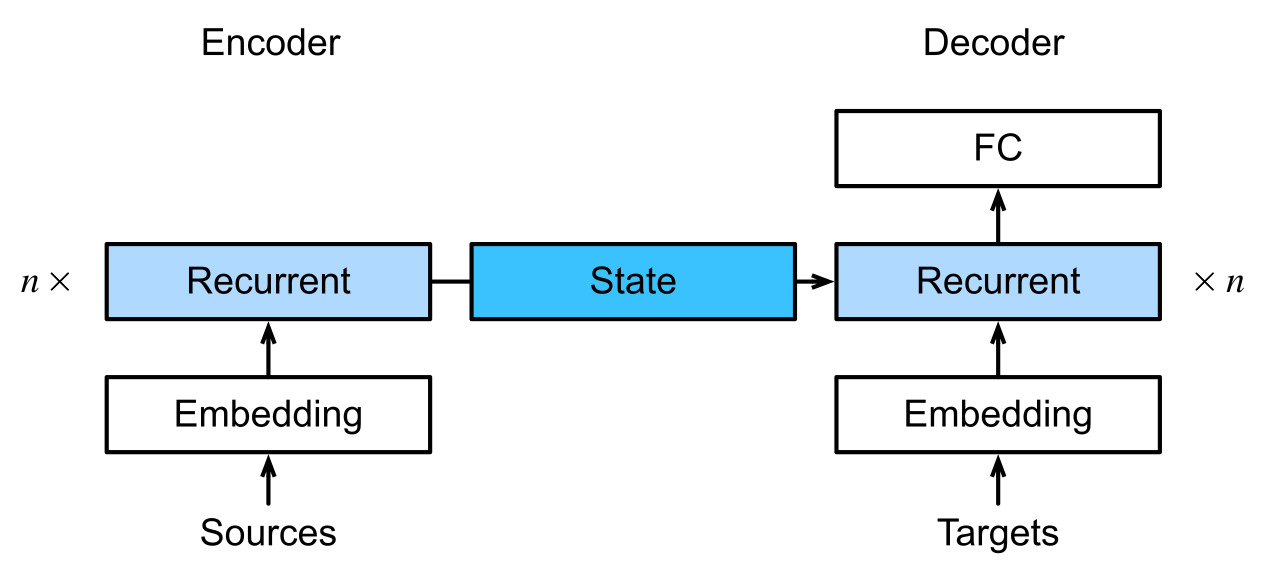
\includegraphics[width=\linewidth, height=3cm, keepaspectratio]{Pictures/deep_neural_networks/seq2seq-state.jpg}
            \caption*{Sequence-to-sequence model. The state, as generated by the encoder, is the only piece of information shared between the encoder and the decoder.}
        \end{figure}
    \end{minipage}
    \hfill
    \begin{minipage}{0.49\linewidth}
        \begin{figure}[H]
            \centering
            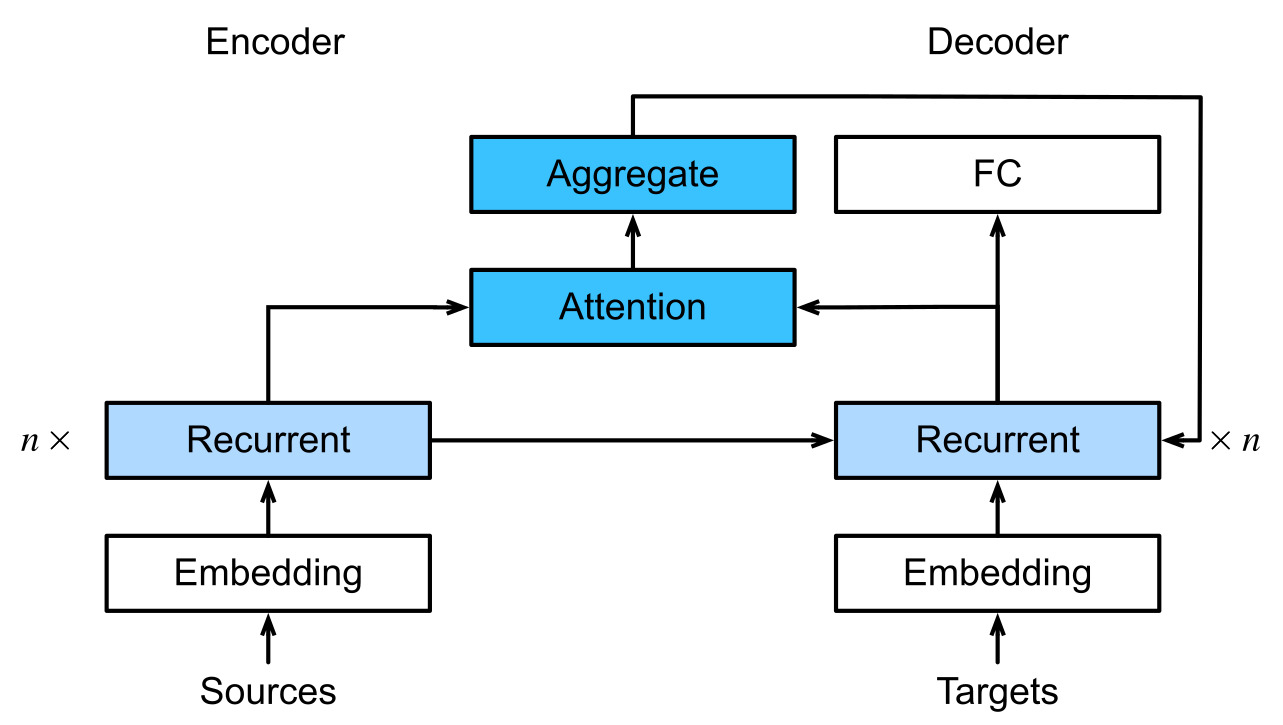
\includegraphics[width=\linewidth, height=3.5cm, keepaspectratio]{Pictures/deep_neural_networks/seq2seq-details-attention.jpg}
            \caption*{Layers in an RNN encoder–decoder model with the Bahdanau attention mechanism}
        \end{figure}
    \end{minipage}
\end{table}

\begin{enumerate}
    \item Conventionally, in an RNN all relevant information about a source sequence is translated into some internal fixed-dimensional state representation by the encoder. 
    
    \item It is this very state that is used by the decoder as the complete and exclusive source of information for generating the translated sequence. 
    
    \item In other words, the sequence-to-sequence mechanism treats the intermediate state as a sufficient statistic of whatever string might have served as input.

    \item While this is quite reasonable for short sequences, it is clear that it is infeasible for long ones

    \item After all, before too long there will simply not be enough “space” in the intermediate representation to store all that is important in the source sequence.
    
    \item Consequently the decoder will fail to translate long and complex sentences.

    \item a differentiable attention model without the unidirectional alignment limitation. 
    
    \item When predicting a token, if not all the input tokens are relevant, the model aligns (or attends) only to parts of the input sequence that are deemed relevant to the current prediction. \\
    This is then used to update the current state before generating the next token.

    
\end{enumerate}


\subsection*{Model \cite{dnn-1}}

\begin{customTableWrapper}{1.5}
\begin{longtable}{l p{8cm}}
    $\mathbf{c}$ & context variable summarizing the source sentence (fixed) \\

    $T$ & input sequence length \\

    $t'$ & time step \\

    $\mathbf{h}_{t}$ & encoder hidden states \\

    $\mathbf{s}_{t'-1}$ & decoder hidden states \\

    $\alpha$ & attention weight \\

\end{longtable}
\end{customTableWrapper}

\begin{enumerate}[itemsep=0.15cm]
    \item $\mathbf{c}_{t'} = \dsum_{t=1}^{T} \alpha(\mathbf{s}_{t' - 1}, \mathbf{h}_{t}) \mathbf{h}_{t}$

    \item The key idea is that instead of keeping the state, i.e., the context variable $\mathbf{c}$ summarizing the source sentence, as fixed, we dynamically update it, as a function of both the original text (encoder hidden states $\mathbf{h}_{t}$) and the text that was already generated (decoder hidden states $\mathbf{s}_{t'-1}$).

    \item We used $\mathbf{s}_{t' - 1}$ as the query, and $\mathbf{h}_{t}$ as both the key and the value.

    \item $\mathbf{c}_{t'}$ is then used to generate the state $\mathbf{s}_{t'}$ and to generate a new token (SEE: \fullref{rnn: Decoder})

    \item In particular, the attention weight $\alpha$ is computed using the additive attention scoring function
    \begin{enumerate}
        \item \fullref{Dot Product Attention}
        \item \fullref{Additive Attention}
    \end{enumerate}

    \item Note that later this model was modified so as to include the already generated tokens in the decoder as further context (i.e., the attention sum does not stop at $T$ but rather it proceeds up to $t'-1$)

    
\end{enumerate}

\subsection{Decoder with Attention \cite{dnn-1}} \label{Decoder with Attention}

\begin{enumerate}
    \item The state of the decoder is initialized with 
    \begin{enumerate}
        \item the hidden states of the last layer of the encoder at all time steps, used as keys and values for attention; 
        
        \item the hidden state of the encoder at all layers at the final time step, which serves to initialize the hidden state of the decoder; and 
    
        \item the valid length of the encoder, to exclude the padding tokens in attention pooling. 

    \end{enumerate}
    
    
    \item At each decoding time step, the hidden state of the final layer of the decoder, obtained at the previous time step, is used as the query of the attention mechanism. 
    
    \item Both the output of the attention mechanism and the input embedding are concatenated to serve as the input of the RNN decoder.

\end{enumerate}





\section{Multi-Head Attention \cite{dnn-1}} \label{Multi-Head Attention}

\begin{figure}[H]
    \centering
    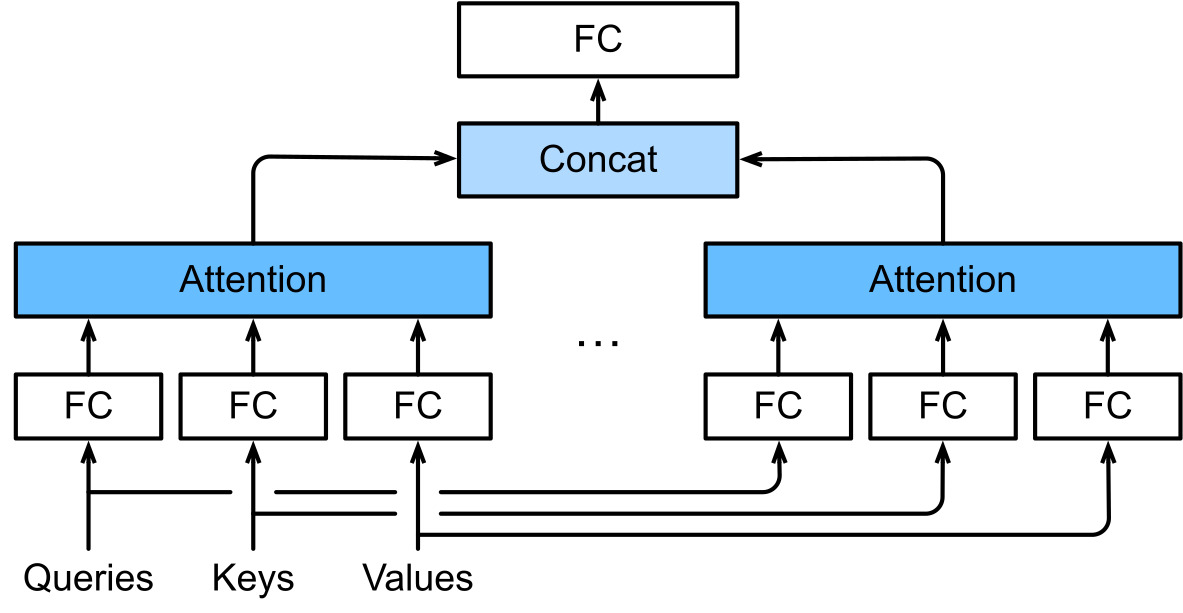
\includegraphics[width=\linewidth, height=3cm, keepaspectratio]{Pictures/deep_neural_networks/multi-head-attention.jpg}
    \caption*{Multi-head attention, where multiple heads are concatenated then linearly transformed}
\end{figure}


\begin{enumerate}
    \item In practice, given the same set of queries, keys, and values we may want our model to combine knowledge from different behaviors of the same attention mechanism, such as capturing dependencies of various ranges (e.g., shorter-range vs. longer-range) within a sequence. 
    
    \item Thus, it may be beneficial to allow our attention mechanism to jointly use different representation subspaces of queries, keys, and values

    \item instead of performing a single attention pooling, queries, keys, and values can be transformed with $h$ independently learned linear projections. \\
    Then these $h$ projected queries, keys, and values are fed into attention pooling in parallel.\\
    In the end, $h$ attention-pooling outputs are concatenated and transformed with another learned linear projection to produce the final output.\\
    This design is called multi-head attention, where each of the $h$ attention pooling outputs is a head.\\
    Using fully connected layers to perform learnable linear transformations.


\end{enumerate}


\subsection*{Model \cite{dnn-1}}

\begin{customTableWrapper}{1.5}
\begin{longtable}{l p{8cm}}
    $\mathbf{q} \in \mathbb{R}^{d_q}$ & query \\

    $\mathbf{k} \in \mathbb{R}^{d_k}$ & key \\

    $\mathbf{v} \in \mathbb{R}^{d_v}$ & value \\

    $\mathbf W_i^{(q)}\in\mathbb R^{p_q\times d_q}$ & (learnable parameter) \\

    $\mathbf W_i^{(k)}\in\mathbb R^{p_k\times d_k}$ & (learnable parameter) \\

    $\mathbf W_i^{(v)}\in\mathbb R^{p_v\times d_v}$ & (learnable parameter) \\

    $f$ & attention pooling, such as additive attention and scaled dot product attention \\

    $\mathbf{h}_i$ & attention head $(i = 1, \ldots, h)$ \\

    $\mathbf W_o\in\mathbb R^{p_o\times h p_v}$ & \\
\end{longtable}
\end{customTableWrapper}

\begin{enumerate}[itemsep=0.15cm]
    \item $\mathbf{h}_i = f(\mathbf W_i^{(q)}\mathbf q, \mathbf W_i^{(k)}\mathbf k,\mathbf W_i^{(v)}\mathbf v) \in \mathbb R^{p_v}$

    \item The multi-head attention output is another linear transformation via learnable parameters $\mathbf W_o$ of the concatenation of $h$ heads:
    $
        \mathbf W_o \begin{bmatrix}\mathbf h_1\\\vdots\\\mathbf h_h\end{bmatrix} \in \mathbb{R}^{p_o}
    $

    \item Based on this design, each head may attend to different parts of the input.\\
    More sophisticated functions than the simple weighted average can be expressed.
\end{enumerate}








\section*{Additional References}

\begin{enumerate}
    \item Attention for Neural Networks, Clearly Explained!!!\\
    \url{https://www.youtube.com/watch?v=PSs6nxngL6k}

    \item The Attention Mechanism in Large Language Models\\
    \url{https://www.youtube.com/watch?v=OxCpWwDCDFQ}

    \item The math behind Attention: Keys, Queries, and Values matrices\\
    \url{https://www.youtube.com/watch?v=UPtG_38Oq8o}

    
\end{enumerate}







